\documentclass[12pt]{article}
\linespread{1}

% margins
\setlength{\textwidth}{6.5in}
\setlength{\textheight}{8.75in}
\setlength{\oddsidemargin}{-0.1in}
\setlength{\topmargin}{-0.1in}
\setlength{\baselineskip}{10pt}

% load packages
\usepackage{amsmath}
\usepackage{amsfonts}
\usepackage{lscape}
\usepackage[round]{natbib}
\usepackage{graphicx}
\graphicspath{{figures_old/}{figures/}{figures_old/roc}{figures_old/calibration_curves}}
\usepackage{amssymb}
\usepackage{color}
\usepackage{hyperref}
\usepackage{booktabs}
\usepackage{verbatim}

% style setup
\bibliographystyle{plainnat}
\pagestyle{empty}
\setlength\parindent{0pt}
\setlength{\parskip}{\baselineskip}

% new commands
\newcommand{\indist}{\overset{d}{\rightarrow}}
\newcommand{\inprob}{\overset{P}{\rightarrow}}
\newcommand{\tabby}{\hspace{10pt}}
\newcommand{\ones}{{\bf 1}}
\newcommand{\tp}{\intercal}
\newcommand{\iprod}[2]{\langle #1 , #2 \rangle}

\newcommand{\note}[1]{\textcolor{red}{#1}}

% header
\title{HOSEA project report}
\author{Simon Fontaine}
\date{\today}

\begin{document}

%\maketitle


\begin{figure}[h]
\centering
\includegraphics[width=0.45\textwidth]{figures/pdp_new/age.pdf}
\includegraphics[width=0.45\textwidth]{figures/shap_new/age.pdf}
\end{figure}
\begin{figure}[h]
\centering
\includegraphics[width=0.45\textwidth]{figures/pdp_new/bmi.pdf}
\includegraphics[width=0.45\textwidth]{figures/shap_new/bmi.pdf}
\end{figure}
\begin{figure}[h]
\centering
\includegraphics[width=0.45\textwidth]{figures/pdp_new/weight.pdf}
\includegraphics[width=0.45\textwidth]{figures/shap_new/weight.pdf}
\end{figure}
\begin{figure}[h]
\centering
\includegraphics[width=0.45\textwidth]{figures/pdp_new/gender.pdf}
\includegraphics[width=0.45\textwidth]{figures/shap_new/gender.pdf}
\end{figure}
\begin{figure}[h]
\centering
\includegraphics[width=0.45\textwidth]{figures/pdp_new/black.pdf}
\includegraphics[width=0.45\textwidth]{figures/shap_new/black.pdf}
\end{figure}
\begin{figure}[h]
\centering
\includegraphics[width=0.45\textwidth]{figures/pdp_new/smoke_current.pdf}
\includegraphics[width=0.45\textwidth]{figures/shap_new/smoke_current.pdf}
\end{figure}
\begin{figure}[h]
\centering
\includegraphics[width=0.45\textwidth]{figures/pdp_new/smoke_former.pdf}
\includegraphics[width=0.45\textwidth]{figures/shap_new/smoke_former.pdf}
\end{figure}





\begin{figure}[h]
\centering
\includegraphics[width=0.45\textwidth]{figures/pdp_new/copd.pdf}
\includegraphics[width=0.45\textwidth]{figures/shap_new/copd.pdf}
\end{figure}
\begin{figure}[h]
\centering
\includegraphics[width=0.45\textwidth]{figures/pdp_new/gerd.pdf}
\includegraphics[width=0.45\textwidth]{figures/shap_new/gerd.pdf}
\end{figure}




\begin{figure}[h]
\centering
\includegraphics[width=0.45\textwidth]{figures/pdp_new/wbc_tv.pdf}
\includegraphics[width=0.45\textwidth]{figures/shap_new/wbc_tv.pdf}
\end{figure}
\begin{figure}[h]
\centering
\includegraphics[width=0.45\textwidth]{figures/pdp_new/wbc_mean.pdf}
\includegraphics[width=0.45\textwidth]{figures/shap_new/wbc_mean.pdf}
\end{figure}
\begin{figure}[h]
\centering
\includegraphics[width=0.45\textwidth]{figures/pdp_new/wbc_min.pdf}
\includegraphics[width=0.45\textwidth]{figures/shap_new/wbc_min.pdf}
\end{figure}
\begin{figure}[h]
\centering
\includegraphics[width=0.45\textwidth]{figures/pdp_new/wbc_max.pdf}
\includegraphics[width=0.45\textwidth]{figures/shap_new/wbc_max.pdf}
\end{figure}
\begin{figure}[h]
\centering
\includegraphics[width=0.45\textwidth]{figures/pdp_new/wbc_mindiff.pdf}
\includegraphics[width=0.45\textwidth]{figures/shap_new/wbc_mindiff.pdf}
\end{figure}
\begin{figure}[h]
\centering
\includegraphics[width=0.45\textwidth]{figures/pdp_new/wbc_maxdiff.pdf}
\includegraphics[width=0.45\textwidth]{figures/shap_new/wbc_maxdiff.pdf}
\end{figure}







\end{document}
